%%%%%%%%%%%%%%%%%%%%%%%%%%%%%%%%%%%%%%%%%%%%%%%%%%%%%%%%%%%%%%%%%%%%%%%%%%%%
%% Trim Size: 9.75in x 6.5in
%% Text Area: 8in (include Runningheads) x 5in
%% ws-ijmpa.tex   :   06-04-2015
%% Tex file to use with ws-ijmpa.cls written in Latex2E.
%% The content, structure, format and layout of this style file is the
%% property of World Scientific Publishing Co. Pte. Ltd.
%% Copyright 2015 by World Scientific Publishing Co.
%% All rights are reserved.
%%%%%%%%%%%%%%%%%%%%%%%%%%%%%%%%%%%%%%%%%%%%%%%%%%%%%%%%%%%%%%%%%%%%%%%%%%%%
%%

%\documentclass[draft]{ws-ijmpa}
\documentclass{ws-ijmpa}
\usepackage[super,compress]{cite}
\usepackage{graphicx}
\begin{document}
\markboth{Authors' Names}{Instructions for typing manuscripts (paper's title)}

%%%%%%%%%%%%%%%%%%%%% Publisher's Area please ignore %%%%%%%%%%%%%%%
%
\catchline{}{}{}{}{}
%
%%%%%%%%%%%%%%%%%%%%%%%%%%%%%%%%%%%%%%%%%%%%%%%%%%%%%%%%%%%%%%%%%%%%

\title{Where in the world in New Physics ?}

\author{Yasmine Amhis\footnote{
Typeset names in 8 pt roman, uppercase. Use the footnote to indicate the
present or permanent address of the author.}
}

\address{University Department, University Name, Address\\
City, State ZIP/Zone, Country\footnote{
State completely without abbreviations, the affiliation and
mailing address, including country. Typeset in 8 pt italic.}\\
first\_author@domain\_name}

\author{Viola Sordini}

\address{Group, Laboratory, Address\\
City, State ZIP/Zone, Country\\
second\_author@domain\_name}

\maketitle

\begin{history}
\received{Day Month Year}
\revised{Day Month Year}
\end{history}

\begin{abstract}
Bananas, melonas

\keywords{Keyword1; keyword2; keyword3.}
\end{abstract}

\ccode{PACS numbers:}

%\tableofcontents

\section{General Appearance}	

Contributions to {\it International Journal of Modern Physics A}
are to be in American English. Authors are encouraged to have their
contribution checked for grammar. American spelling should be
used. Abbreviations are allowed but should be spelt out in full when
first used. Integers ten and below are to be spelt out.  Italicize
foreign language phrases (e.g.~Latin, French).  Upon acceptance,
authors are required to submit their data source file including
postscript files for figures.

The text is to be typeset in 10 pt roman, single spaced with
baselineskip of 13~pt. Text area (including copyright block)
is 8 inches high and 5 inches wide for the first page.  Text area
(excluding running title) is 7.7 inches high and 5 inches wide for
subsequent pages.  Final pagination and insertion of running titles
will be done by the publisher.

\section{Running Heads}

Please provide a shortened runninghead (not more than eight words) for
the title of your paper. This will appear on the top right-hand side
of your paper.

\section{Major Headings}

Major headings should be typeset in boldface with the first
letter of important words capitalized.

\subsection{Subheadings}

Subheadings should be typeset in boldface italic and capitalize
the first letter of the first word only. Section number to be in
boldface roman.

\subsubsection{Subsubheadings}

Typeset subsubheadings in medium face italic and capitalize the
first letter of the first word only. Section numbers to be in
roman.

\subsection{Numbering and spacing}

Sections, subsections and subsubsections are numbered in
Arabic.  Use double spacing before all section headings, and
single spacing after section headings. Flush left all paragraphs
that follow after section headings.

\subsection{Lists of items}

Lists may be laid out with each item marked by a dot:
\begin{itemlist}
 \item item one,
 \item item two.
\end{itemlist}
Items may also be numbered in lowercase roman numerals:
\begin{romanlist}[(ii)]
\item item one,
\item item two.
	\begin{romanlist}[(b)]
	\item Lists within lists can be numbered with lowercase
              roman letters,
	\item second item.
	\end{romanlist}
\end{romanlist}

\section{Equations}

Displayed equations should be numbered consecutively in each
section, with the number set flush right and enclosed in
parentheses
\begin{equation}
\mu(n, t) = \frac{\sum^\infty_{i=1} 1(d_i < t, N(d_i)
= n)}{\int^t_{\sigma=0} 1(N(\sigma) = n)d\sigma}\,.
\label{diseqn}
\end{equation}

Equations should be referred to in abbreviated form,
e.g.~``Eq.~(\ref{diseqn})'' or ``(2)''. In multiple-line
equations, the number should be given on the last line.

Displayed equations are to be centered on the page width.
Standard English letters like x are to appear as $x$
(italicized) in the text if they are used as mathematical
symbols. Punctuation marks are used at the end of equations as
if they appeared directly in the text.

\section{Theorem Environments}

\begin{theorem}
Theorems$,$ lemmas$,$ propositions$,$ corollaries are to be numbered
consecutively in the paper or in each section. Use italic for the
body and upper and lower case boldface$,$ for the declaration.
\end{theorem}

\begin{remark}
Remarks, examples, definitions are to be numbered
consecutively in the paper or in each section. Use roman for the
body and upper and lower case boldface$,$ for the declaration.
\end{remark}

\begin{proof}
The word `Proof' should be type in boldface. Proofs
should end with\break
a box.
\end{proof}

\section{Figures}

Figures are to be embedded in the text nearest their first reference
and sequentially numbered in Arabic numerals. The caption must be
placed below the figure (see Fig.~\ref{f1}) and typeset in 8 pt roman with
baselineskip of 10 pt. Use double spacing between a caption and the
text that follows immediately.

\begin{figure}[b]
\centerline{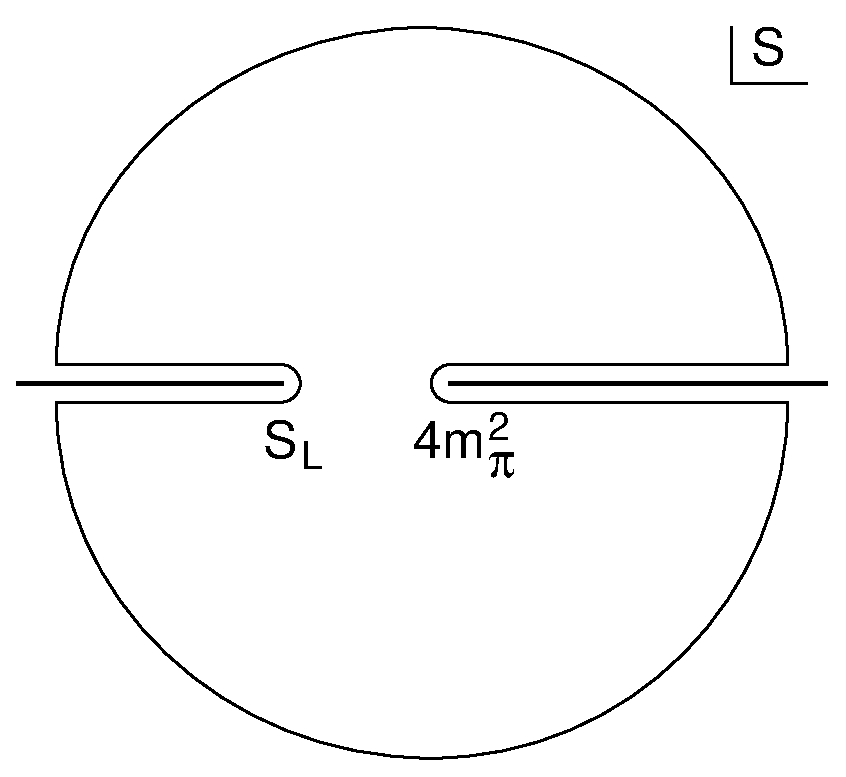
\includegraphics[width=3.8cm]{ijmpaf1}}
\caption{A schematic illustration of dissociative recombination. The
direct mechanism, 4m$^2_\pi$ is initiated when the
molecular ion S$_{\rm L}$ captures an electron with
kinetic energy. \label{f1}}
\end{figure}

Figures should be black and white (or half-tone) and of a good
resolution and sharpness. Compressed formats, such as JPEG, should not
use heavy compression, which introduces undesirable artifacts. Bitmap
figures, such as photographs or half-tone images, should be at least
300 dpi (TIFF, BMP or JPEG). Vector (line-art) figures, such as
charts and technical drawings, should be 600--1200 dpi (EPS, PS,
PDF). The native formats of software packages will not be permitted.

Previously published material must be accompanied by written
permission from the author and publisher.

\section{Tables}

Tables should be inserted in the text as close to the point of
reference as possible. Some space should be left above and below
the table.

Tables should be numbered sequentially in the text in Arabic
numerals. Captions are to be centralized above the tables (see
Table~\ref{ta1}).  Typeset tables and captions in 8 pt roman with
baselineskip of 10 pt.

\begin{table}[ph]
\tbl{Comparison of acoustic for frequencies for piston-cylinder problem.}
{\begin{tabular}{@{}cccc@{}} \toprule
Piston mass & Analytical frequency & TRIA6-$S_1$ model &
\% Error \\
& (Rad/s) & (Rad/s) \\ \colrule
1.0\hphantom{00} & \hphantom{0}281.0 & \hphantom{0}280.81 & 0.07 \\
0.1\hphantom{00} & \hphantom{0}876.0 & \hphantom{0}875.74 & 0.03 \\
0.01\hphantom{0} & 2441.0 & 2441.0\hphantom{0} & 0.0\hphantom{0} \\
0.001 & 4130.0 & 4129.3\hphantom{0} & 0.16\\ \botrule
\end{tabular} \label{ta1}}
\end{table}

If tables need to extend over to a second page, the continuation of
the table should be preceded by a caption, e.g.~``{\it Table 2.}
$(${\it Continued}$)$''.

\section{Footnotes}

Footnotes should be numbered sequentially in superscript
lowercase roman letters.\footnote{Footnotes should be
typeset in 8 pt roman at the bottom of the page.}

\section{About References and their Formats}

References are to be listed in the order cited in the text in Arabic
numerals. They should be listed according to the style shown in the
References. Typeset references in 9 pt roman.

It is recommended that each cited publication is labeled with a unique reference number. Format that contains multiple/grouped citations, e.g. ``A. David, {\it Int. J. Phys.} {\bf 18}, 11150 (2000); {\bf 18}, 22350 (2003); J. John, {\it ibid.} {\bf 6}, 11204 (2010)'', is not encouraged.

References in the text can be typed in superscripts,
e.g.: ``$\ldots$ have proven\cite{autbk,edbk,rvo} that
this equation $\ldots$'' or after punctuation marks:
``$\ldots$ in the statement.\cite{rvo}'' This is
done using LaTeX command: ``\verb|\cite{name}|''.

When the reference forms part of the sentence, it should not
be typed in superscripts, e.g.: ``One can show from
Ref.~\refcite{autbk} that $\ldots$'', ``See
Refs.~\citen{jpap,colla,autbk}, \refcite{rvo}
and \refcite{pro} for more details.''
This is done using the LaTeX
command: ``Ref.~\verb|\citen{name}|''.

\section*{Acknowledgments}

This section should come before the References. Dedications and funding
information may also be included here.

\appendix

\section{Appendices}

Appendices should be used only when absolutely necessary. They
should come before the References. If there is more than one
appendix, number them alphabetically. Number displayed equations
occurring in the Appendix in this way, e.g.~(\ref{app1}),\break
(\ref{app2}), etc.
\begin{eqnarray}	%A.1
\begin{array}{rcl}
g_{\mu_1\mu_2} &=& g_{axby}=-\displaystyle{\epsilon_{abc}}{4\pi}\,
\frac{(x-y)^c}{|x-y|^3}\,, \\[8pt]
h_{\mu_1\mu_2\mu_3} &=& \epsilon^{\alpha_1 \alpha_2 \alpha_3}
g_{\mu_1\alpha_1}g_{\mu_2\alpha_2}g_{\mu_3\alpha_3}
\end{array}
\label{app1}
\end{eqnarray}
with
\begin{eqnarray}	%A.2
\epsilon^{\alpha_1 \alpha_2 \alpha_3} = \epsilon^{b_1y_1b_2y_2cx} =
\epsilon^{b_1b_2c}\delta(x-y_1)\delta(x-y_2)\,.
\label{app2}
\end{eqnarray}

%\begin{thebibliography}{000} %for 3 digits
%\begin{thebibliography}{00}  %for 2 digits
\begin{thebibliography}{0}    %for 1 digit

%%journal paper
\bibitem{jpap} R. Loren and D. B. Benson, {\it J. Comput.
System Sci.} {\bf 27}, 400 (1983).

\bibitem{lee} M. Lee, {\it Int. J. Phys.} {\bf 18}, 255 (2010) [Erratum: {\it ibid.} {\bf18}, 440 (2010)].

%%collaboration
\bibitem{colla} OPAL Collab. (G. Abbiendi {\it et al}.),
{\it Eur. J. Phys. C\/} {\bf 11}, 217 (1999).

%%normal book (authors)
\bibitem{autbk} R. Loren and D. B. Benson, {\it Introduction to String
Field Theory}, 2nd edn. (Springer-Verlag, New York, 1999).

%%normal book (editors)
\bibitem{edbk} R. Loren and D. B. Benson (eds.), {\it Introduction to
String Field Theory}, 2nd edn. (Springer-Verlag, New York, 1999).

%%review volume
\bibitem{rvo} C. M. Wang, J. N. Reddy and K. H. Lee, New set of
buckling parameters, in {\it Shear Deformable Beams}, ed.~T. Rex
(Elsevier, Oxford, 2000), p.~201.

%%book in a series
\bibitem{seri} R. Loren, J. Li and D. B. Benson, Deterministic flow-chart
interpretations, in {\it Introduction to String Field Theory},
Ad. Series in Math. Phys., Vol.~3 (Springer-Verlag, New York, 1999),
p.~401.

%%proceedings
\bibitem{pro} R. Loren, J. Li and D. B. Benson, Deterministic
flow-chart interpretations, in {\it Proc. 3rd Int. Conf.
Entity-Relationship Approach}, eds. C. G. Davis and R. T. Yeh
(North-Holland, Amsterdam, 1983), p.~421.

%%to be published
\bibitem{publ} R. Loren, J. Li and D. B. Benson, Deterministic
flow-chart interpretations, to appear in {\it J. Comput. System Sci.}
\end{thebibliography}
\end{document}